\documentclass{article}
\usepackage{graphicx}
\usepackage[T1]{fontenc}
% LTeX: language=es
\usepackage[spanish]{babel}
\graphicspath{ {./resources/} }
\usepackage{float}
\usepackage{listings}
\usepackage{xcolor}
\usepackage{subfigure}
\usepackage{hyperref}

\definecolor{codegreen}{rgb}{0,0.6,0}
\definecolor{codegray}{rgb}{0.5,0.5,0.5}
\definecolor{codepurple}{rgb}{0.58,0,0.82}
\definecolor{backcolour}{rgb}{0.95,0.95,0.92}

\lstdefinestyle{mystyle}{
    backgroundcolor=\color{backcolour},   
    commentstyle=\color{codegreen},
    keywordstyle=\color{magenta},
    numberstyle=\tiny\color{codegray},
    stringstyle=\color{codepurple},
    basicstyle=\ttfamily\footnotesize,
    breakatwhitespace=false,         
    breaklines=true,                 
    captionpos=b,                    
    keepspaces=true,                 
    showspaces=false,                
    showstringspaces=false,
    showtabs=false,                  
    tabsize=2
}

\begin{document}

\section{Introducción}

La siguiente guía de instalación busca guiar al usuario en la configuración básica de un laboratorio de Oracle Real Application Clusters, esta guía no busca enseñarle al usuario a utilizar Linux, pero si buscara proporcionar un poco de contexto adicional sobre ciertos comandos de Unix. El laboratorio utiliza 3 máquinas virtuales, las cuales usaran Linux con distribuciones basadas en Ubuntu y RHEL, por otro lado el sistema operativo puede ser cualquiera de preferencia por el usuario, pero en este caso se usará Pop\_Os!, el cual se encuentra basado en Ubuntu.

\section{Configuración de Máquinas Virtuales}

El primer paso consiste en preparar nuestras máquinas virtuales para los nodos de Oracle DB, estos usarán Oracle Linux 7 con Oracle DB 19c, acá cada nodo tiene cuenta con los siguientes requerimientos.

\begin{itemize}
	\item 4 GB de memoria RAM.
	\item 100 GB de almacenamiento físico.
	\item 2 núcleos de procesamiento.
\end{itemize}

Empezando con la creación del primer nodo en este cluster sera llamado ``node1'', aparte de las especificaciones ya mencionadas es necesario crear 3 adaptadores de red:

\begin{itemize}
	\item ``Host-only Adapter'': Usado para conectar à la base de datos hacia otros aplicativos.
	\item ``Internal Network Adapter'': Usado por la red interna del clúster.
	\item ``Bridged Adapter'': Usado para conectarse hacia el internet, usando al sistema operativo huésped.
\end{itemize}

\begin{figure}[H]
	\begin{center}
		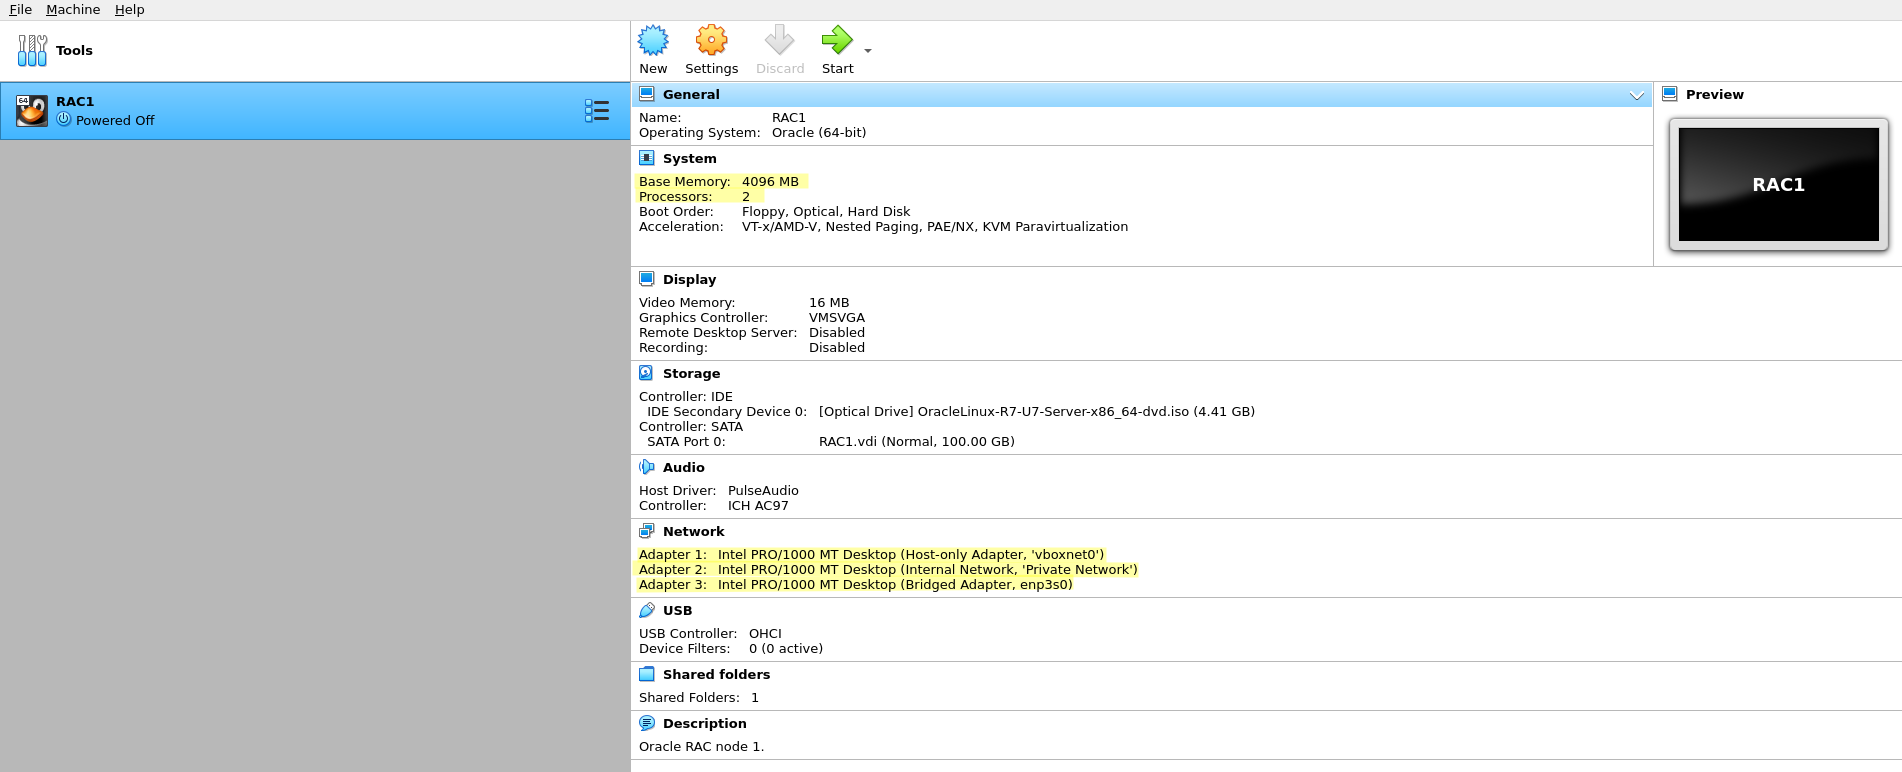
\includegraphics[width=0.95\textwidth]{vm_base.png}
	\end{center}
	\caption{Pantalla de inicio de Configuración de la Máquina Virtual}
\end{figure}

Al momento de iniciar la máquina virtual e insertar el archivo ISO con Oracle Linux 7, podemos empezar a configurar la instalación del sistema operativo. Acá iniciaremos con la configuración de partición del disco desde acá se selecciona ``Installation Destination'', en donde se puede ver el disco creado y las opciones de particiones, acá se seleccionará ``I will configure Partitioning''. Acá crearemos las siguientes particiones.

\begin{center}
	\begin{tabular}{ |c|c|c| }
		\hline
		\multicolumn{2}{|c|}{Lista de Particiones}    \\
		\hline
		Nombre de Partición & Capacidad               \\
		\hline
		/boot               & 2 GB de almacenamiento  \\
		/root               & 5 GB de almacenamiento  \\
		/ o root            & 50 GB de almacenamiento \\
		/swap               & 8 GB de almacenamiento  \\
		\hline
	\end{tabular}
\end{center}

Al volver al menú de inicio de nuestro instalador, se selecciona el software por instalar en nuestra nueva instalación, acá se selecciona la opción ``Software Selection'', acá se puede escoger entre varios ambientes, pero se seleccionará ``Server with GUI'' con los siguientes paquetes de software.

\begin{itemize}
	\item ``Hardware Monitoring Utilities''
	\item ``Large Systems Performance''
	\item ``Network file system client''
	\item ``Performance Tools''
	\item ``Compatibility Libraries''
	\item ``Development Tools''
\end{itemize}

Al volver al inicio del instalador se puede configurar las opciones de red en ``Network and Hostname'' para configurar los adaptadores de red instalados en las máquinas virtuales. 

Después de habilitar el primer adaptador de red, seleccione ``Configure'' y en la pestaña de ``ipv4'' se usara la dirección IP ``192.168.24.1/24'' con una salida de ``0.0.0.0''  manualmente.

\begin{figure}[H]
	\begin{center}
		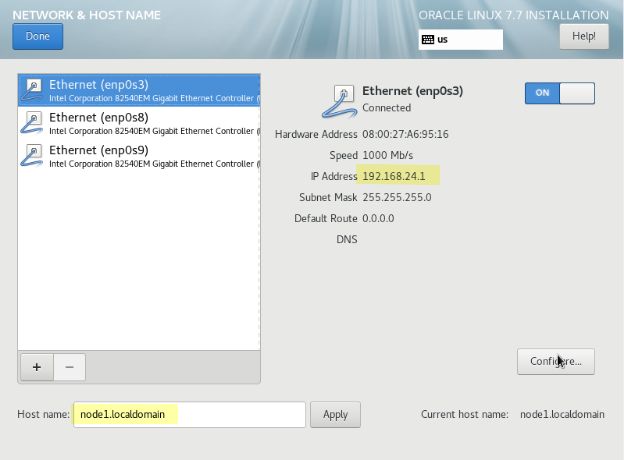
\includegraphics[width=0.95\textwidth]{vm_networking.png}
	\end{center}
	\caption{Configuración de Red de la Instalación de Oracle Linux}
\end{figure}

Se aplicará esta misma configuración manual en el siguiente adaptador disponible, pero esta vez con una dirección IP de ``192.168.10.1/24'' con una salida de ``0.0.0.0'', finalmente para el último adaptador habilitaremos direccionamiento automático con DHCP. Se puede continuar con la instalación del sistema operativo, en la siguiente pantalla podemos seleccionar una contraseña para el usuario ``sudo'', para este ejercicio se usará ``root'' como contraseña.

\section{Configuración del Sistema Operativo}

El siguiente paso consiste en preparar al sistema operativo para la instalación de los componentes de Oracle Grid y Oracle DB.

\subsection{Instalación de Paquetes}

Una vez en el ambiente de escritorio es necesario instalar software mediante el gestor de paquetes, en este caso esta distribución se encuentra basada en RHEL así que el gestor de paquete es yum.

\begin{lstlisting}[style=mystyle,language=bash]
	$ sudo yum update
	$ sudo yum install -y oracle-database-preinstall-19c.x86_64
	$ sudo yum install oracleasm-support
	$ sudo yum install bind* --skip-broken
\end{lstlisting}

\subsection{Configuración de Red}

Siguiente se configurara el archivo de hosts, según Verhage (2021) este archivo ubicado en \texttt{etc/host} se encarga de conectar direcciones ip con nombre de dominio.

\begin{lstlisting}[style=mystyle,language=bash]
	cat /etc/hosts
	127.0.0.1   	localhost
	::1         	localhost
	127.0.1.1   	pop-os.localdomain  	pop-os
\end{lstlisting}

En este caso, al visitar la dirección \texttt{127.0.0.1}, nuestro sistema operativo le indicará al navegador que debe de navegar hacia \texttt{localhost}. Para esto se puede abrir el editor de texto predeterminado del sistema operativo, gedit, o simplemente un editor de texto de consola, en este caso vim ya viene instalado. Aca se agregaran los siguientes cambios.

\begin{lstlisting}[style=mystyle,language=bash]
	# Default
	127.0.0.1   localhost localhost.localdomain localhost4 localhost4.localdomain4
	::1     	localhost localhost.localdomain localhost6 localhost6.localdomain6
	# Public
	192.168.24.1 node1.localdomain node1
	192.168.24.2 node2.localdomain node2
	# Private
	192.168.10.1 node-priv.localdomain node1-priv
	192.168.10.2 node2-priv.localdomain node2-priv
	# Virtual
	192.168.24.31 node1-vip.localdomain node1-vip
	192.168.24.32 node2-vip.localdomain node2-vip
	# SCAN
	192.168.24.41 node-scan.localdomain node-scan
	192.168.24.42 node-scan.localdomain node-scan
	192.168.24.43 node-scan.localdomain node-scan
\end{lstlisting}

Acá se esta mapeando los nombres de dominio con las redes a las cuales pertenece cada adaptador de red con el cual cuenta la máquina virtual, por esto mismo las direcciones proporcionadas se encuentran en la misma red.

\subsection{Configuración de Usuarios}

El uso de usuarios y grupos de usuarios permite restringir el acceso de estos sobre los distintos archivos en el sistema operativo, esto nos permitirá controlar su acceso sobre cualquier parte del sistema operativo, ya que la filosofía UNIX indica que ``todo es un archivo'' (ArchWiki, n.d.). Según la Wiki de ArchLinux (n.d) se puede crear a un nuevo usuario y grupo de usuarios con los siguientes comandos de consola:

\begin{lstlisting}[style=mystyle,language=bash]
	useradd John
	groupadd Accountants
\end{lstlisting}

Y para asignar entonces a un usuario a un grupo de usuarios se puede usar el siguiente comando de consola.

\begin{lstlisting}[style=mystyle,language=bash]
	useradd John
	groupadd Accountants
\end{lstlisting}

Con este contexto se puede crear a los grupos de usuarios requeridos para instalar la base de datos y configurar RAC.

\begin{lstlisting}[style=mystyle,language=bash]
	groupadd -g 54327 asmdba
	groupadd -g 54328 asmoper
	groupadd -g 54329 asmadmin
\end{lstlisting}

Aca la bandera \texttt{-g} permite asignar un identificador a cada grupo de usuario, podemos entonces verificar el contenido del archivo \texttt{/etc/group} para ver a los usuarios creados y sus grupos correspondientes.

\begin{lstlisting}[style=mystyle,language=bash]
	cat /etc/group | grep asm
	asmdba:x:54327:
	asmoper:x:54328:
	asmadmin:x:54329:
\end{lstlisting}

Estos nuevos usuarios tienen que pertenecer al grupo ya existente oracle, así que se va a modificar su grupo principal.

\begin{lstlisting}[style=mystyle,language=bash]
	usermod -G asmdba,asmoper,asmadmin oracle
\end{lstlisting}

Según Amoany (2021) podemos modificar la contraseña de un usuario con el comando \texttt{passwd}, en donde un usuario puede modificar únicamente su propia contraseña y un super-usuario puede modificar la contraseña de cualquier otro usuario en el sistema. Con este comando se modificara la contraseña para el usuario ya existente oracle.

\begin{lstlisting}[style=mystyle,language=bash]
	sudo passwd oracle
	[sudo] password for node1:
	Changing password for user oracle.
	New password:
	Retype new password:
	passwd: all authentication tokens updated successfully.
\end{lstlisting}

\subsection{Configuración de Directorios}

Siguiente se crearan los directorios necesarios para instalar el software de oracle, para esto se usara el comando mkdir, desde el directorio \texttt{root}. También se modificará al dueño del directorio y sus permisos con los comandos \texttt{chown} y \texttt{chmod}.

\begin{lstlisting}[style=mystyle,language=bash]
	mkdir -p /u01/app/19c/grid
	mkdir -p /u01/app/oracle/product/19c/db_1
	chown -R oracle:oinstall /u01
	chmod -R 775 /u01/
\end{lstlisting}

Entonces para verificar los permisos en este directorio se puede utilizar al comando \texttt{ls} y unas banderas adicionales.

\begin{lstlisting}[style=mystyle,language=bash]
	ls -al /u01
	total 4
	drwxrwxr-x.  3 oracle oinstall   17 Oct 27 23:11 .
	dr-xr-xr-x.  18 root   root 	4096 Oct 27 23:11 ..
	drwxrwxr-x.  4 oracle oinstall   31 Oct 27 23:12 app
\end{lstlisting}

Según la ArchWiki (n.d) en la primera columna se pueden ver los permisos que sobre este directorio o archivo, en este caso el usuario tiene permisos de lectura, escritura y ejecución (rwx), los usuarios que pertenecen al grupo del usuario actual tiene permisos de lectura, escritura y ejecución (rwx), finalmente otros usuarios solo tienen permisos de lectura y ejecución (r-x), en la tercera y cuarta columna se puede ver al usuario actual y grupo dueño de este archivo, aca el directorio actual es propiedad del usuario oracle y del grupo oinstal.

\subsection{Configuración de Variables de Ambiente}

Para preparar la instalación de Grid y Oracle DB, se iniciará sesión como el usuario oracle, su contraseña fue configurada previamente, acá se van a configurar varias variables de ambiente en el ambiente. Acá nuestro sistema operativo incluye bash, por lo cual podemos modificar nuestras variables de ambiente modificando el archivo \texttt{\.bash\_profile} ubicado en el directorio home, por referencia su ruta es: \texttt{/home/oracle/\.bash\_profile}. Este será modificado con los siguientes cambios:

\begin{lstlisting}[style=mystyle,language=bash]
	# Oracle Settings
	export TMP=/tmp
	export TMPDIR=$TMP
	export ORACLE_BASE=/u01/app/oracle
	export GRID_HOME=/u01/app/19c/grid
	export DB_HOME=$ORACLE_BASE/product/19c/db_1
	export ORACLE_HOME=$DB_HOME
	export ORACLE_SID=node1
	export ORACLE_TERM=xterm
	export BASE_PATH=/usr/sbin:$PATH
	export PATH=$ORACLE_HOME/bin:$BASE_PATH
	export LD_LIBRARY_PATH=$ORACLE_HOME/lib:/lib:/usr/lib
	export CLASSPATH=$ORACLE_HOME/JRE:$ORACLE_HOME/jlib:$ORACLE_HOME/rdbms/jlib
	alias grid=’. /home/oracle/grid.env’
	alias db=’. /home/oracle/db.env’
\end{lstlisting}

Siguiente se crearan unos cuantos archivos de ambiente, primero se creara al archivo \texttt{grid\.env} en el directorio \texttt{/home/oracle/} con el siguiente contenido.

\begin{lstlisting}[style=mystyle,language=bash]
	export ORACLE_SID=+ASM1
	export ORACLE_HOME=$GRID_HOME
	export PATH=$ORACLE_HOME/bin:$BASE_PATH
	export LD_LIBRARY_PATH=$ORACLE_HOME/lib:/lib:/usr/lib
	export CLASSPATH=$ORACLE_HOME/JRE:$ORACLE_HOME/jlib:$ORACLE_HOME/rdbms/jlib
\end{lstlisting}

Siguiente se creará al archivo \texttt{db.env} en el directorio \texttt{/home/oracle/} con el siguiente contenido.

\begin{lstlisting}[style=mystyle,language=bash]
	export ORACLE_SID=node1
	export ORACLE_HOME=$DB_HOME
	export PATH=$ORACLE_HOME/bin:$BASE_PATH
	export LD_LIBRARY_PATH=$ORACLE_HOME/lib:/lib:/usr/lib
	export CLASSPATH=$ORACLE_HOME/JRE:$ORACLE_HOME/jlib:$ORACLE_HOME/rdbms/jlib
\end{lstlisting}

Estos dos archivos incluyen las variables de ambiente tanto para Grid y Oracle DB.

\subsection{Deshabilitar el Firewall}

Para la instalación de Oracle y Grid es necesario deshabilitar el firewall de nuestro sistema operativo, es posible ponerlo en línea después de terminar con la instalación.

\begin{lstlisting}[style=mystyle,language=bash]
	systemctl stop firewalld.service
	systemctl disable firewalld.service
\end{lstlisting}

Para estas operaciones es necesario que proporcionar las credenciales del usuario sudo.

\subsection{Sincronización del Reloj}

Los nodos necesitan sincronizar los relojes entre sí, para esto existe el protocolo NTP (ArchWiki, n.d), entonces sera necesario habilitar este servicio en el nodo con los siguientes comandos.

\begin{lstlisting}[style=mystyle,language=bash]
	systemctl enable chronyd.service
	systemctl restart chronyd.service
	chronyc -a burst 4/4
	chronyc -a makestep
\end{lstlisting}

Acá primero se habilita y reinicia el servicio de \texttt{chrony}, una implementación del protocolo NTP, mediante su proceso de fondo \texttt{chronyd}, por otro lado se modifica la configuración de \texttt{chronyc} con la línea de comando \texttt{chronyc}.
Con el comando burst de chronyc le indicamos a chrony el mínimo de buenas medidas para sincronizar con otro nodo. Con la opción makestep le indicamos a chrony que en caso de que los nodos se encuentren desincronizados, que realice correcciones inmediatas en el nodo.

\subsection{Clonado de la Máquina Virtual}

Con la configuración básica de la máquina virtual se puede clonar a la máquina virtual para crear a otro nodo en la red.

\begin{figure}[H]
	\begin{center}
		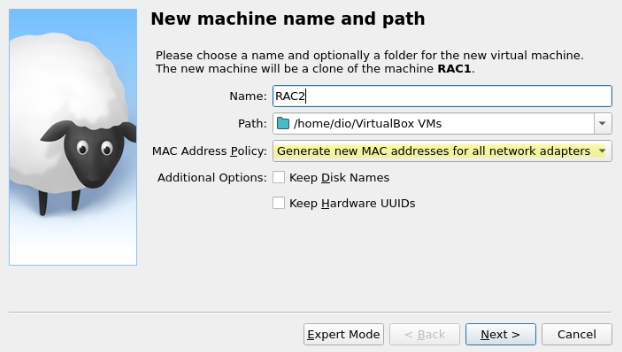
\includegraphics[width=0.95\textwidth]{vm_clone.png}
	\end{center}
	\caption{Clonado de la Máquina Virtual}
\end{figure}

Con este nuevo nodo creado, puede ya ser iniciado y se cambiará su nombre o hostname a ``node2'', ya que este es el nombre es el indicado para el primer nodo al momento de configurar \texttt{/etc/hosts}, para cambiar el \texttt{hostname} de una máquina se utiliza el comando \texttt{nmcli}, primero se verificara cuál es el nombre de dominio actual.

\begin{lstlisting}[style=mystyle,language=bash]
	$ hostname
	node1.localdomain
	$ nmcli general hostname node2.localdomain
	$ hostname
	node2.localdomain
\end{lstlisting}

Con esto listo, aún tenemos que cambiar las direcciones IP en nuestras interfaces de red para que se puedan comunicar con el otro nodo en la red. Con este cambio se puede iniciar el primer nodo y hacer un \texttt{ping} entre los dos.

\subsection{Creación de Discos Compartidos}

Oracle RAC comparte al mismo juego de discos, para simular esto, se creará un disco compartido entre máquinas virtuales. En la pestaña de almacenamiento de la máquina virtual se puede crear un nuevo disco.

\begin{figure}[H]
		\begin{center}
			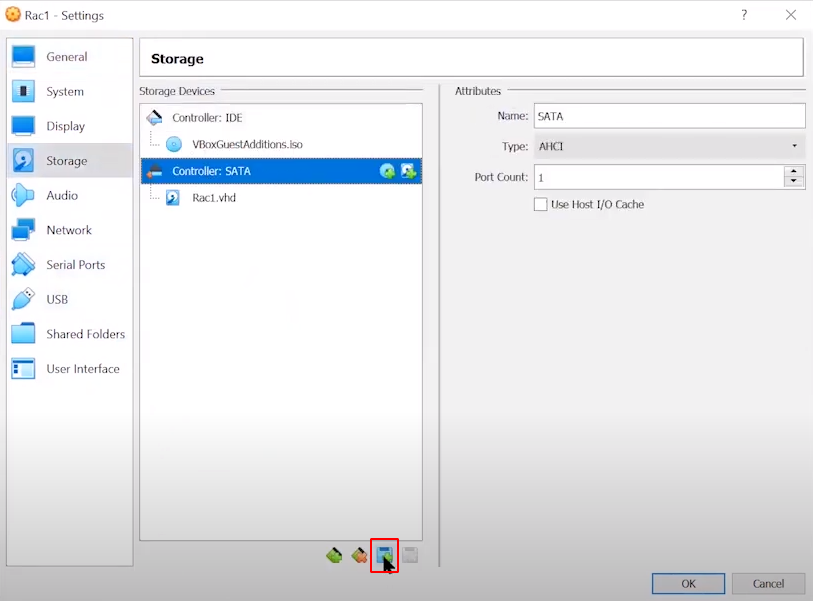
\includegraphics[width=0.95\textwidth]{vm_shared_disk_creation.png}
		\end{center}
		\caption{Creación de Discos Compartidos}
\end{figure}

Acá seleccioné la opción ``Create''.

\begin{figure}[H]
		\begin{center}
			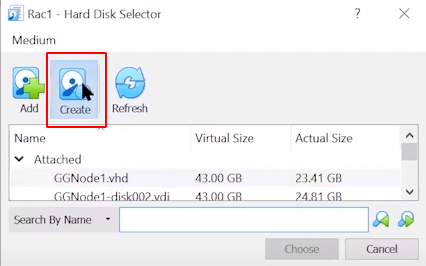
\includegraphics[width=0.95\textwidth]{vm_shared_disk_create.png}
		\end{center}
		\caption{Creación de un Nuevo Disco}
\end{figure}

Para el tipo de disco seleccioné VHD o ``Virtual Hard Disk''.

\begin{figure}[H]
		\begin{center}
			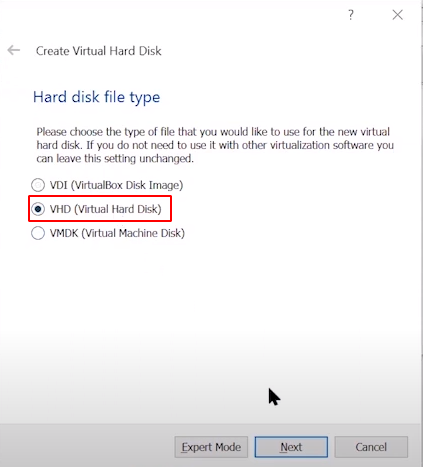
\includegraphics[width=0.95\textwidth]{vm_shared_disk_creation_type.png}
		\end{center}
		\caption{Tipo de Disco por Crear}
\end{figure}

Finalmente seleccioné una ubicación de preferencia para almacenar el archivo y el nombre de este.

\begin{figure}[H]
		\begin{center}
			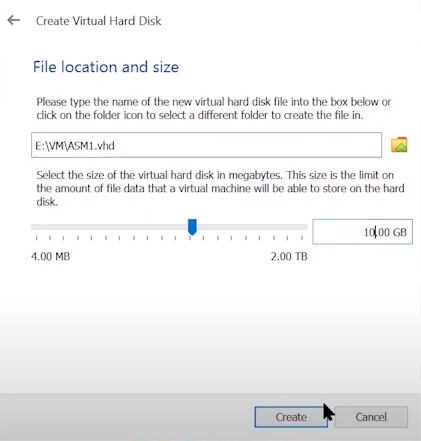
\includegraphics[width=0.95\textwidth]{vm_shared_disk_creation_location.png}
		\end{center}
		\caption{Ubicación del Disco por Crear}
\end{figure}

Este mismo proceso debería ser creado hasta que se obtengan los siguientes discos.

\begin{figure}[H]
		\begin{center}
			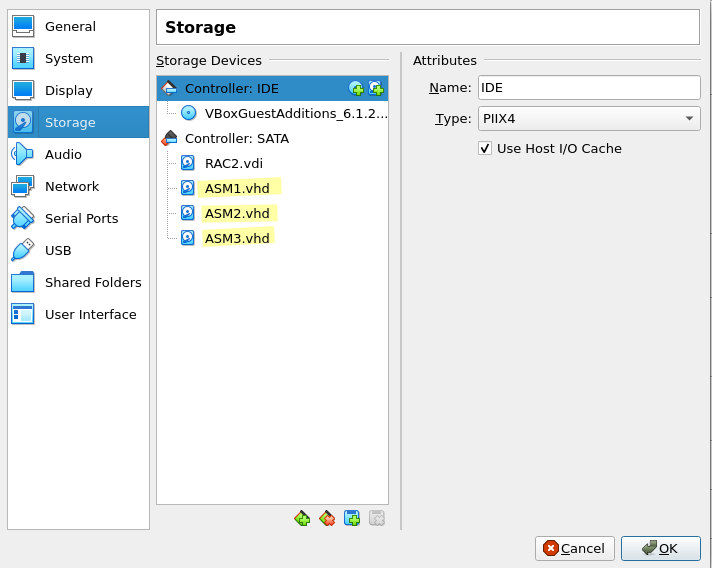
\includegraphics[width=0.95\textwidth]{vm_shared_disk_result.png}
		\end{center}
		\caption{Creación de Discos Compartidos Resultado}
\end{figure}

En la segunda máquina virtual en el diálogo para agregar nuevos discos, solo es necesario seleccionar los discos ya creados.

\begin{figure}[H]
		\begin{center}
			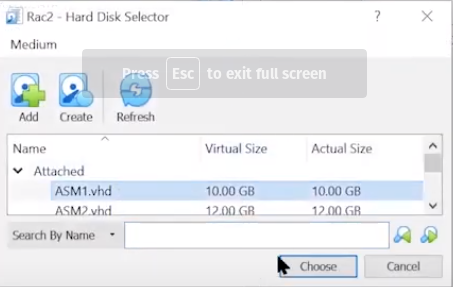
\includegraphics[width=0.95\textwidth]{vm_shared_disk_mounting.png}
		\end{center}
		\caption{Montar un Disco ya Creado}
\end{figure}

Con los discos ya montados en ambos nodos, se puede iniciar cualquiera de los nodos y para verificar si los discos se encuentran disponibles con el siguiente comando.

\begin{lstlisting}[style=mystyle,language=bash]
	$ ls /dev/sd*
	/dev/sda  /dev/sda1  /dev/sda2  /dev/sdb  /dev/sdc  /dev/sdd
\end{lstlisting}

Acá se encuentran a los discos \texttt{sdb}, \texttt{sdc} y \texttt{sdd}, estos con los discos que se acaban de montar, pero estos aun no se encuentran formateados, para esto usaremos el comando \texttt{fdisk}, esto ejecutara un programa interactivo para crear nuevas particiones en el disco.

\begin{lstlisting}[style=mystyle,language=bash]
	$ fdisk /dev/sdb
	Welcome to fdisk (util-linux 2.23.2).

	Changes will remain in memory only, until you decide to write them.
	Be careful before using the write command.

	Device does not contain a recognized partition table
	Building a new DOS disklabel with disk identifier 0x28e162da.

	Command (m for help): n
	Partition type:
	   p   primary (0 primary, 0 extended, 4 free)
	   e   extended
	Select (default p): p
	Partition number (1-4, default 1): 1
	First sector (2048-20971519, default 2048):
	Using default value 2048
	Last sector, +sectors or +size{K,M,G} (2048-20971519, default 20971519):
	Using default value 20971519
	Partition 1 of type Linux and of size 10 GiB is set
	Command (m for help): w
	The partition table has been altered!

	Calling ioctl() to re-read partition table.
	Syncing disks.
\end{lstlisting}

Después de esto si se vuelve a verificar a los discos montados se obtiene la siguiente salida.

\begin{lstlisting}[style=mystyle,language=bash]
	$ ls /dev/sd*
	/dev/sda  /dev/sda1  /dev/sda2  /dev/sdb  /dev/sdb1  /dev/sdc  /dev/sdd
\end{lstlisting}

Acá se encuentra una partición nueva \texttt{/dev/sdb1}, si se repite este proceso con los 2 discos faltantes se obtiene entonces el siguiente resultado.

\begin{lstlisting}[style=mystyle,language=bash]
	$ ls /dev/sd*
	/dev/sda  /dev/sda1  /dev/sda2  /dev/sdb  /dev/sdb1  /dev/sdc  /dev/sdc1  /dev/sdd  /dev/sdd1
\end{lstlisting}

\subsection{Configuración de Discos para ASM}

Siguiente se pueden preparar los discos para su uso en \texttt{ASM}, para esto se puede utilizar el comando \texttt{oracleasm configure -i} para iniciar un programa interactivo de configuración.

\begin{lstlisting}[style=mystyle,language=bash]
	$ sudo oracleasm configure -i
	Configuring the Oracle ASM library driver.

	This will configure the on-boot properties of the Oracle ASM library
	driver.  The following questions will determine whether the driver is
	loaded on boot and what permissions it will have.  The current values
	will be shown in brackets ('[]').  Hitting <ENTER> without typing an
	answer will keep that current value.  Ctrl-C will abort.

	Default user to own the driver interface []: oracle
	Default group to own the driver interface []: oinstall
	Start Oracle ASM library driver on boot (y/n) [n]: y
	Scan for Oracle ASM disks on boot (y/n) [y]: y
	Writing Oracle ASM library driver configuration: done
\end{lstlisting}

Siguiente se montará \texttt{ASM} al sistema.

\begin{lstlisting}[style=mystyle,language=bash]
	$ sudo oracleasm init
	Creating /dev/oracleasm mount point: /dev/oracleasm
	Loading module "oracleasm": oracleasm
	Configuring "oracleasm" to use device physical block size
	Mounting ASMlib driver filesystem: /dev/oracleasm
\end{lstlisting}

Con \texttt{ASM} ya montado al sistema, se puede crear un disco este, acá se utilizarán los discos que fueron formateados previamente.

\begin{lstlisting}[style=mystyle,language=bash]
	$ sudo oracleasm createdisk DISK1 /dev/sdb1
	Writing disk header: done
	Instantiating disk: done
\end{lstlisting}

Con el disco ya creado podemos buscarlo y listarlo.

\begin{lstlisting}[style=mystyle,language=bash]
	$ sudo oracleasm scandisks
	Reloading disk partitions: done
	Cleaning any stale ASM disks...
	Scanning system for ASM disks...
	$ oracleasm listdisks
	DISK1
\end{lstlisting}

Solo resta iniciar la otra máquina virtual y configurar \texttt{ASM}, únicamente será necesario omitir la creación del disco.

\subsection{Copiar el Directorio de Instalación de Grid}

Siguiente es necesario descargar Grid y Oracle DB 19c, estos pueden ser descargados desde él \hyperlink{https://www.oracle.com/in/database/technologies/oracle19c-linux-downloads.html}{sitio oficial de Oracle} como zips, entonces se debe de configurar un directorio compartido entre las máquinas virtuales y el sistema operativo huésped.

\begin{figure}[H]
		\begin{center}
			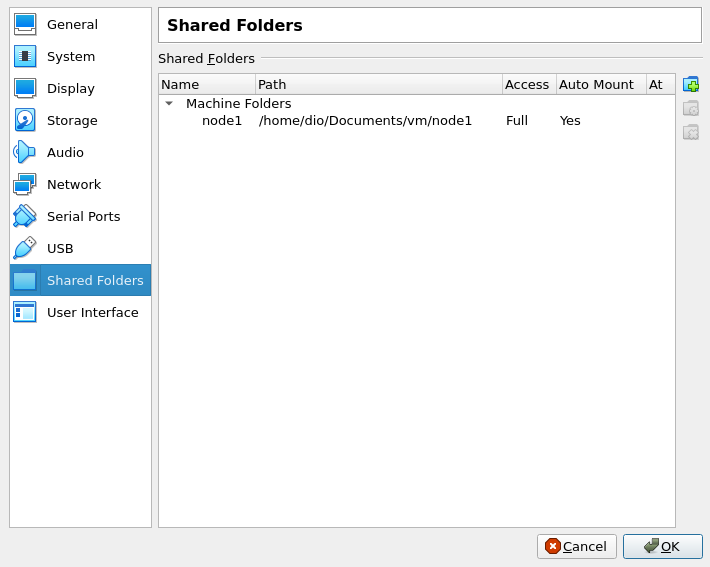
\includegraphics[width=0.95\textwidth]{vm_shared_folder.png}
		\end{center}
		\caption{VirtualBox Carpetas Compartidas}
\end{figure}

En este directorio compartido se deben descargar los dos zips con el software por instalar, luego en la máquina virtual se puede copia hacia el directorio \texttt{/u01/software} y se modifican los permisos sobre este.

\begin{lstlisting}[style=mystyle,language=bash]
	$ df -h 
	Filesystem           Size  Used Avail Use% Mounted on
	shared               916G  141G  775G  16% /media/sf_shared
	… omitido
	$ cd /media
	$ sudo cp sf_shared/LINUX.X64_193000_grid_home /u01/
	$ mkdir software
	$ mv LINUX.X64_193000_grid_home/ software/
	$ chown -P oracle:oinstall software/
	$ chmod -R 775 software/ 
	$ chown -R oracle:oinstall software/
	$ ls -lrt 
	total 0
	drwxrwxr-x. 4 oracle oinstall 31 Oct 27 23:12 app
	drwxrwxr-x. 3 oracle oinstall 40 Nov  2 21:55 software
\end{lstlisting}

\section{Instalación de Componentes de Software}

Con la configuración básica es posible instalar los componentes de software de Oracle en los nodos del cluster.



\end{document}
